\documentclass{beamer}
\usepackage[british]{babel}
\usepackage{times}
\usepackage{amsmath}
\usepackage{mathtools}
\usepackage{amsfonts}
\usepackage{verbatim}
\usepackage{lmodern}
\usepackage{tikz}
\usepackage{graphicx}
\usepackage[ruled,vlined]{algorithm2e}
\usetikzlibrary{patterns}

\usetheme{Frankfurt}

\DeclareMathOperator*{\argmax}{arg\,max}
\DeclareMathOperator*{\argmin}{arg\,min}

\DeclareMathOperator*{\KL}{{\rm KL}}
\DeclareMathOperator*{\const}{{\rm const}}

\newcommand*\mean[1]{\bar{#1}}

\begin{document}
\SetEndCharOfAlgoLine{}

\title{Averaged Variational Inference for Hierarchical Modelling of Genetic Association}
\subtitle{Master thesis}
\author{William van Rooij\\
{\small supervised by Hélène Ruffieux and Anthony Davison}}
\institute{École Polytechnique Fédérale de Lausanne}
\date{09.07.19}
\logo{
\includegraphics[bb=0 0 600 200,width=30px]{images/EPFL_Logo.png}}
\maketitle
\begin{frame}
\begin{itemize}
\item Introduction
\item Hierarchical model
\item Variational inference
\item Methods
\item Simulations
\item Conclusion
\end{itemize}
\end{frame}

\begin{frame}
\frametitle{Introduction}
\begin{itemize}
\item Estimate associations between genetic variants and diseases or phenotypes.
\item The most common genetic variants are single nucleotide polymorphisms (SNPs).
\item SNPs are strongly correlated with a block pattern.
\item Not many observations compared to the number of parameters, i.e., small $n$, large $p$ situation.
\item Traditional techniques do not apply, so we need to find an alternative.
\end{itemize}
\end{frame}

\begin{frame}
\frametitle{Introduction}
\begin{figure}
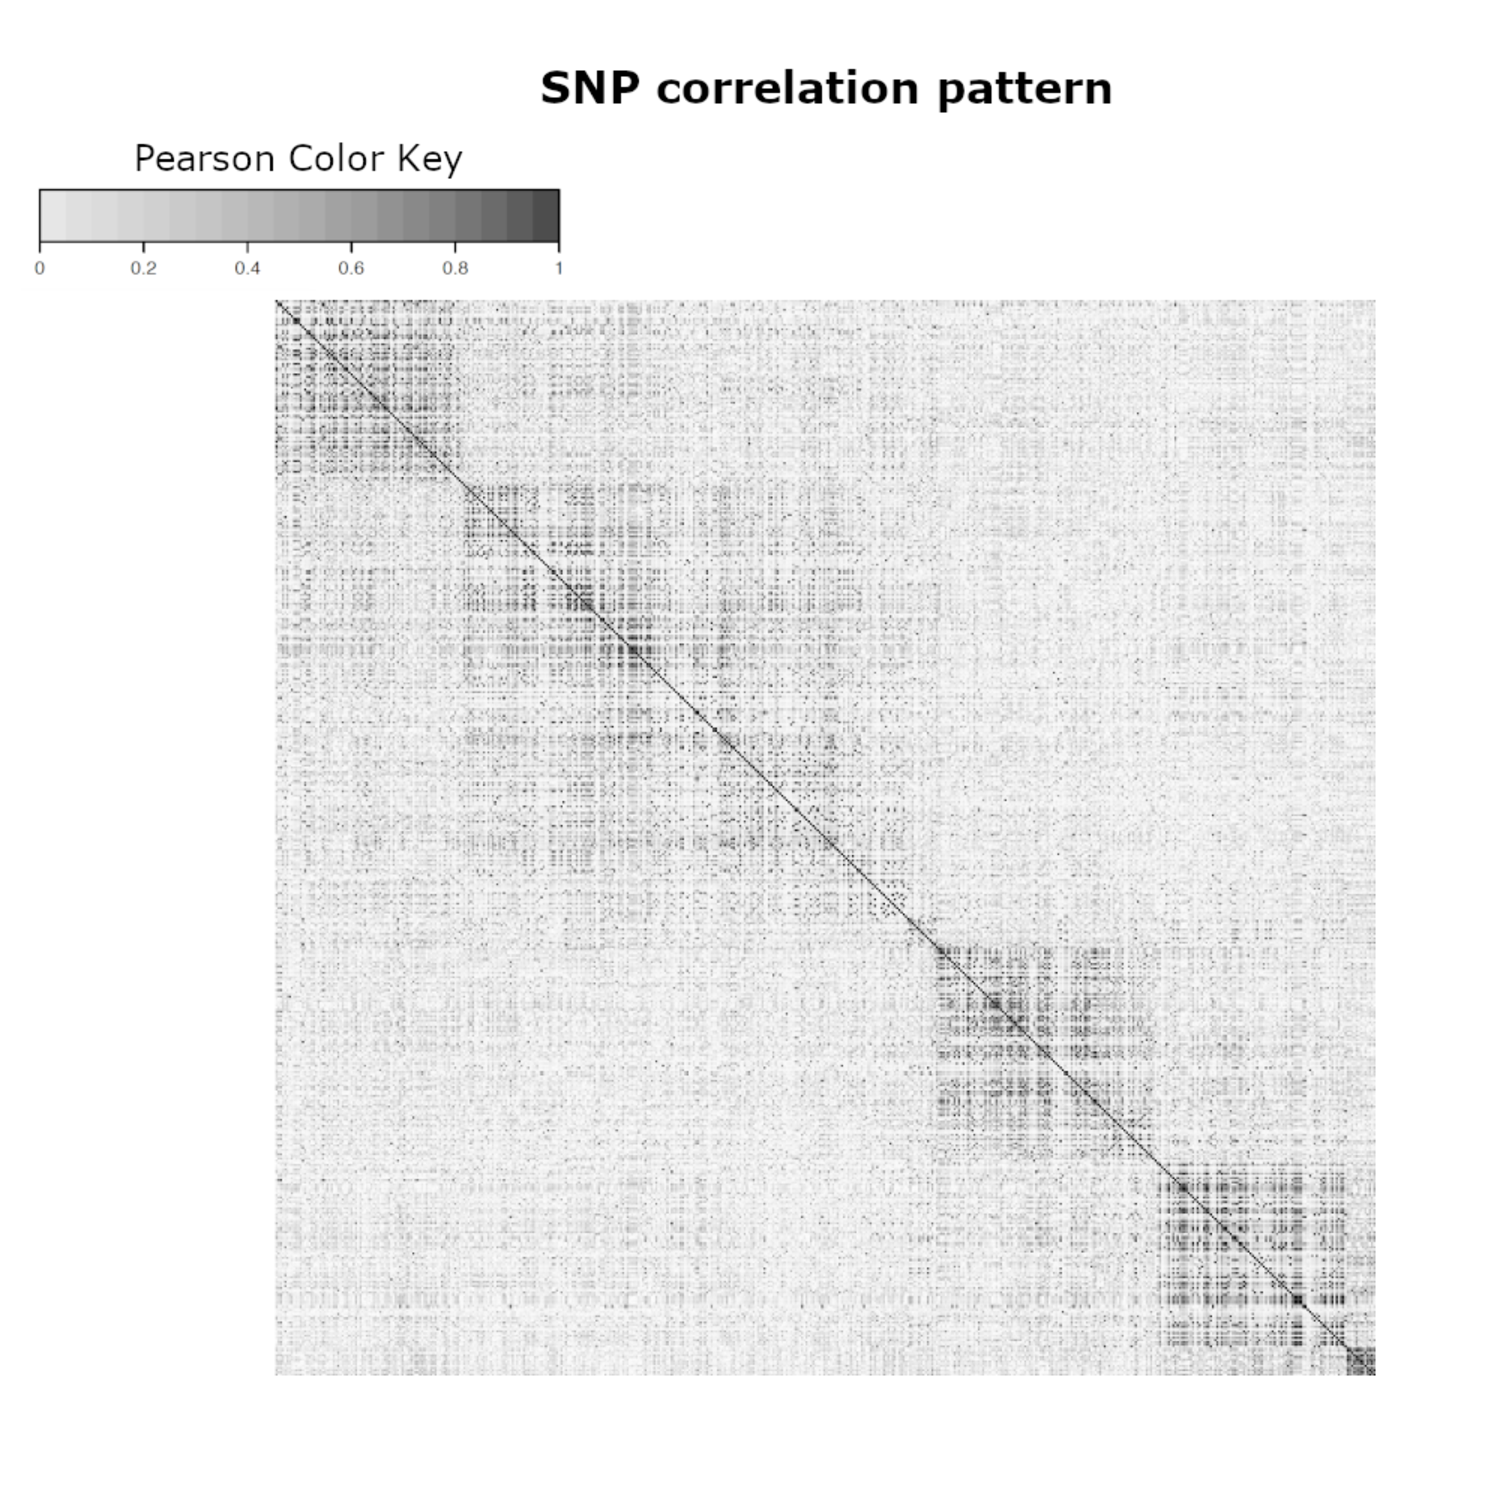
\includegraphics[width=3in]{images/corrRealSNPs.pdf}
\end{figure}
\end{frame}

\begin{frame}
\frametitle{Hierarchical model}
\begin{itemize}
\item We introduce $\boldsymbol{X} = (\boldsymbol{X}_1,\ldots,\boldsymbol{X}_p)$, and $\boldsymbol{y} = (\boldsymbol{y}_1,\ldots,\boldsymbol{y}_q)$,
\item A SNP $\boldsymbol{X}_s$ and a trait $\boldsymbol{y}_t$,
\item Estimate the association between SNP $s$ and trait $t$,
\item For all $s = 1,\ldots,p$, $t=1,\ldots,q$,
\item $\boldsymbol{y}_t \mid \boldsymbol{\beta}_t, \tau_t\; \sim\; \mathcal{N}(\boldsymbol{X\beta}_t,\tau_t^{-1}\boldsymbol{I}_n)$,
\item $\beta_{st}\mid\gamma_{st},\sigma^2,\tau_t\; \sim\; \gamma_{st}\;\mathcal{N}(0,\sigma^2\tau_t^{-1})+(1-\gamma_{st})\;\delta_0$,
\item $\gamma_{st} \mid \omega_{s} \sim $ Bernoulli$(\omega_s)$,
\item $\omega_s \sim $ Beta$(a_s,b_s)$,
\item $a_s, b_s$ chosen to enforce sparsity,
\item $\tau_t$ and $\sigma^{-2}$ have Gamma priors.

\end{itemize}

\end{frame}

\begin{frame}
\frametitle{Hierarchical model}
\begin{itemize}
\item Markov Chain Monte Carlo algorithms (MCMC) are the usual way to approximate inference in relatively small datasets.
\item This is a small $n$, large $p$, large $q$ situation.
\item MCMC gets time consuming, computational cost of operations increases with the number of parameters.
\item Number of iterations needed increases with the number of parameters.
\item Variational inference as an alternative to MCMC inference. 
\end{itemize}
\end{frame}

\begin{frame}
\frametitle{Variational Inference}
\begin{itemize}
\item Observed data $\boldsymbol{y}$, parameters $\boldsymbol{\theta}$, posterior distribution of parameters $p(\boldsymbol{\theta} \mid \boldsymbol{y})$.
\item Approximate the posterior density with a simpler density $q$, minimizing a "closeness" measure: the reverse Kullback--Leibler divergence.
\item $\KL(q\parallel p) := \int q(\boldsymbol{\theta})\log \left\lbrace\dfrac{q(\boldsymbol{\theta})}{p(\boldsymbol{\theta} \mid \boldsymbol{y})}\right\rbrace \mathrm{d}\boldsymbol{\theta}$.
\item $\KL$ difficult to minimize.
\end{itemize}
\end{frame}
\begin{frame}
\frametitle{Variational Inference}
\begin{itemize}
\item Evidence lower bound (ELBO): $\mathcal{L}(q) = \mathbb{E}_q\left[\log p(\boldsymbol{\theta},\boldsymbol{y})\right] - \mathbb{E}_q\left[\log q(\boldsymbol{\theta})\right]$.
\item $\KL(q\parallel p) = \log(p) - \mathcal{L}(q)$.
\item Minimizing KL is equivalent to maximizing ELBO.
\item It is easier to maximize ELBO than to minimize KL.
\end{itemize}
\end{frame}

\begin{frame}
\frametitle{Mean-field approximation}
\begin{itemize}
\item We assume independence for most of the parameters:
$$
q(\boldsymbol{\theta}) = \left\lbrace\prod_{s=1}^p\prod_{t=1}^qq(\beta_{st},\gamma_{st})\right\rbrace\left\lbrace\prod_{s=1}^pq(\omega_s)\right\rbrace\left\lbrace\prod_{t=1}^qq(\tau_t)\right\rbrace q(\sigma^{-2}).
$$
\item The mean-field approximation does not represent the correlations between parameters.
\end{itemize}
\begin{figure}
\centering
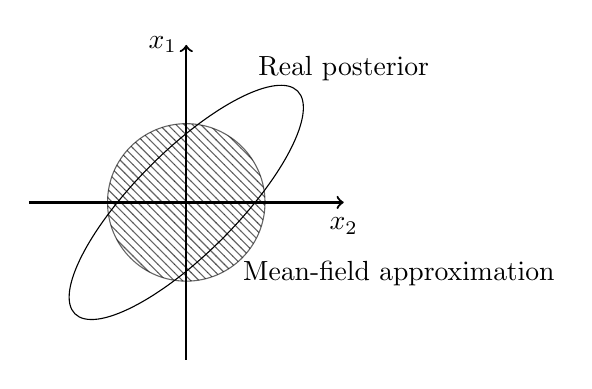
\begin{tikzpicture}
\draw[thick, ->] (0,-2) -- (0,2);
\draw[thick, ->] (-2,0) -- (2,0);
\fill[pattern=north west lines,opacity=.6,draw] (0,0) circle (1cm);
\draw[rotate=-45] (0,0) ellipse (0.65cm and 2cm);
\node (p) at (2,1.7) {Real posterior};
\node (q) at (2.7,-0.9) {Mean-field approximation};
\node (x1) at (-0.3,2) {$x_1$};
\node (x2) at (2,-0.3) {$x_2$};
\end{tikzpicture}\end{figure}
\end{frame}

\begin{frame}
\frametitle{Coordinate ascent variational inference algorithm}
\begin{algorithm}[H]
\SetKwData{ELBO}{$\mathcal{L}(q)$}\SetKwData{OLDELBO}{$\mathcal{L}^{\text{old}}(q)$}
\SetKwFunction{Union}{Union}\SetKwFunction{FindCompress}{FindCompress}
\SetKwInOut{Input}{input}\SetKwInOut{Output}{output}\SetKwInOut{Init}{initialize}
\SetKw{Set}{set}
\Input{$p(\boldsymbol{y},\boldsymbol{\theta})$, dataset $y$, tolerance $\varepsilon$}
\BlankLine
\Output{$q(\boldsymbol{\theta}) = \prod_{j=1}^J q_j(\theta_j)$}
\BlankLine
\Init{the parameters of each $q(\theta_j)$}
\BlankLine
\Repeat{$|$\OLDELBO$-\mathcal{L}(q)| < \varepsilon $}{
\For{$j\in \left\lbrace 1, \ldots, J \right\rbrace $}{
\Set{$q_j(\theta_j) \propto \exp\left\lbrace\mathbb{E}_{-j}\left[\log p(\theta_j \mid \boldsymbol{\theta}_{-j}, \boldsymbol{y})\right]\right\rbrace$}}
\BlankLine
\OLDELBO$\leftarrow$\ELBO\\
\ELBO$\leftarrow\mathbb{E}\left[\log p(\boldsymbol{\theta}, \boldsymbol{y})\right]-\mathbb{E}\left[\log q(\boldsymbol{\theta})\right]$
\BlankLine
}
\Return{$q(\boldsymbol{\theta})$}
\caption{\label{alg:CAVI}Coordinate ascent variational inference}
\end{algorithm}
\end{frame}

%\begin{frame}
%\frametitle{Coordinate ascent variational inference algorithm II}
%\begin{itemize}
%\item $\mathcal{L}(q)$ is guaranteed to increase at every iteration.
%\item We assume there exists a best model and we want to find it
%\item CAVI yields a local optimum, depending on the initialization of the parameters.
%\end{itemize}
%\end{frame}
%
%\begin{frame}
%\frametitle{Parameters posterior distributions}
%\begin{itemize}
%\item $\beta_{st} \mid \gamma_{st} = 1, \boldsymbol{y} \sim \mathcal{N}\left(\mu_{\beta,st},\sigma_{\beta,st}^2\right)$,
%\item $\beta_{st} \mid \gamma_{st} = 0, \boldsymbol{y} \sim \delta_0$,
%\item $\gamma_{st} \mid \boldsymbol{y} \sim $ Bernoulli$(\gamma_{st}^{(1)})$,
%\item $\omega_s \mid \boldsymbol{y} \sim $ Beta$(a^*_s, b^*_s)$,
%\item $\tau_t \mid \boldsymbol{y} \sim $ Gamma$(\eta_t^*, \kappa_t^*)$,
%\item $\sigma^{-2} \mid \boldsymbol{y} \sim $ Gamma$(\lambda^*,\nu^*)$,
%\end{itemize}
%\end{frame}

\begin{frame}
\frametitle{Problem statement}
\begin{itemize}
\item High multimodality of $\mathcal{L}(q)$,
\item mean-field independence assumption,
\item reverse Kullback--Leibler divergence optimization,
\item $\Rightarrow$ variational inference underestimates posterior variances,
\item $\Rightarrow$ tends to concentrate mass on a single mode.
\item Two possibilities:
\begin{enumerate}
\item Simulated annealing,
\item Weighted averaging.
\end{enumerate}
\end{itemize}
\end{frame}

\begin{frame}
\frametitle{Averaged LOCUS}
\begin{itemize}
\item Find the optima $q^*(\boldsymbol{\theta})$ with different initial parameters, drawn at random.
\item Generate the ELBOs and use them as weights in the weighted average.
\item $\mathbb{E}\left[\Delta\mid \boldsymbol{y}\right]= \sum_{k=1}^K \mathbb{E}\left[\Delta\mid M_k,\boldsymbol{y}\right]p(M_k\mid\boldsymbol{y})$
\item The function yields probabilities of association between SNPs and traits.
\end{itemize}
\end{frame}


\begin{frame}
\frametitle{Averaged LOCUS}
\begin{itemize}
\item Denote $M_k$, $k= 1,\ldots, K$ the models yielded by the local optimums.
\item $p(M_k \mid \boldsymbol{y}) = \dfrac{p(\boldsymbol{y} \mid M_k)p(M_k)}{\sum_{j=1}^{K}p(\boldsymbol{y}\mid M_j)p(M_j)},$
\item $\mathcal{L}(q)$ serves as an approximation of $\log p(\boldsymbol{y} \mid M_k)$, as $\KL(q\parallel p) = \log p(\boldsymbol{y}) - \mathcal{L}(q)$.
\item $p(M_k)$ is the prior probability of the models, we consider them to be equiprobable: $p(M_k) = 1/K$, $\forall k = 1,\ldots,K$.
\end{itemize}
\end{frame}

%\begin{frame}
%\frametitle{Annealed LOCUS}
%\begin{itemize}
%\item Temperature $T$, ``smoothing'' the density of interest, and gets lower until initial density is reached. 
%\item Then, perform a standard LOCUS from the reached parameters.
%\item $p_T(\boldsymbol{y},\boldsymbol{\theta}) \propto p(\boldsymbol{y},\boldsymbol{\theta})^{1/T}$,
%\item $\mathcal{L}_T(q_T) = \int q_T(\boldsymbol{\theta}) \log p(\boldsymbol{y},\boldsymbol{\theta})\mathrm{d}\boldsymbol{\theta} - T \int q_T(\boldsymbol{\theta}) \log q_T(\boldsymbol{\theta}) \mathrm{d}\boldsymbol{\theta}$
%
%\end{itemize}
%\begin{align*}
%\mathcal{L}_T(q) &= \mathbb{E}_j\left[\mathbb{E}_{-j}\left\lbrace \log p(\boldsymbol{y},\boldsymbol{\theta})\right\rbrace - T \log q_T(\theta_j)\right]+ \const,\\
%&= T\mathbb{E}_j\left[\log\left\lbrace\frac{p_{T, -j}(\boldsymbol{y}, \theta_j)}{q_T(\theta_j)}\right\rbrace\right] + \const.
%\end{align*}
%
%\end{frame}
%
%\begin{frame}
%\frametitle{Annealed LOCUS II}
%\begin{itemize}
%\item Geometric spacing,
%\begin{equation*}
%T_l = (1 + \Delta)^{l-1},\quad \Delta = T_L^{1/(L-1)}-1,
%\end{equation*}
%
%\item We can combine annealing with the Averaged LOCUS method, which we call Averaged annealed LOCUS.
%\end{itemize}
%\end{frame}
%
%\begin{frame}
%\frametitle{Averaged LOCUS with equal weights}
%\begin{itemize}
%\item Instead of using the lower bound as weights, we average over all the models with equal weights.
%\item $\mathbb{E}\left[\gamma_{st}\mid \boldsymbol{y}\right]=\frac{1}{K} \sum_{k=1}^K \mathbb{E}\left[\gamma_{st}\mid M_k,\boldsymbol{y}\right]$
%\end{itemize}
%\end{frame}

%\begin{frame}
%\frametitle{Expected weights averaged LOCUS}
%\begin{itemize}
%\item Weights depending on the number of associated SNPs
%\item $w_j \propto \exp \left\lbrace-(\#\left[\gamma_{st} > \mean{\gamma}_{st}\right]-p_0)^2\right\rbrace$
%\item $p_0$ is the expected number of associated SNPs per trait $t$.
%\end{itemize}
%\end{frame}

\begin{frame}
\frametitle{Simulations}
\begin{itemize}
\item $n = 300$ observations,
\item $p = 500$ SNPs, with $p_0$ associated SNPs,
\item $q = 1$ trait, %for visualisation
\item $100$ random initialisations,
\item autocorrelation between the SNPs is between $0.95$ and $0.99$, in blocks of ten SNPs,
\item we can specify the maximum proportion of response variance explained by the SNPs.
\item We used $50$ replications to determine the ROC curves.
\end{itemize}
\end{frame}

%\begin{frame}
%\frametitle{LOCUS VS. Averaged LOCUS with $p_0 = 5$, max var. $=0.5$}
%\begin{figure}
%\includegraphics[width=2.1in]{images/s_locus.png}
%\includegraphics[width=2.1in]{images/m_locus.png}
%\end{figure}
%\end{frame}


\begin{frame}
\frametitle{ROC curves comparison}
\begin{figure}
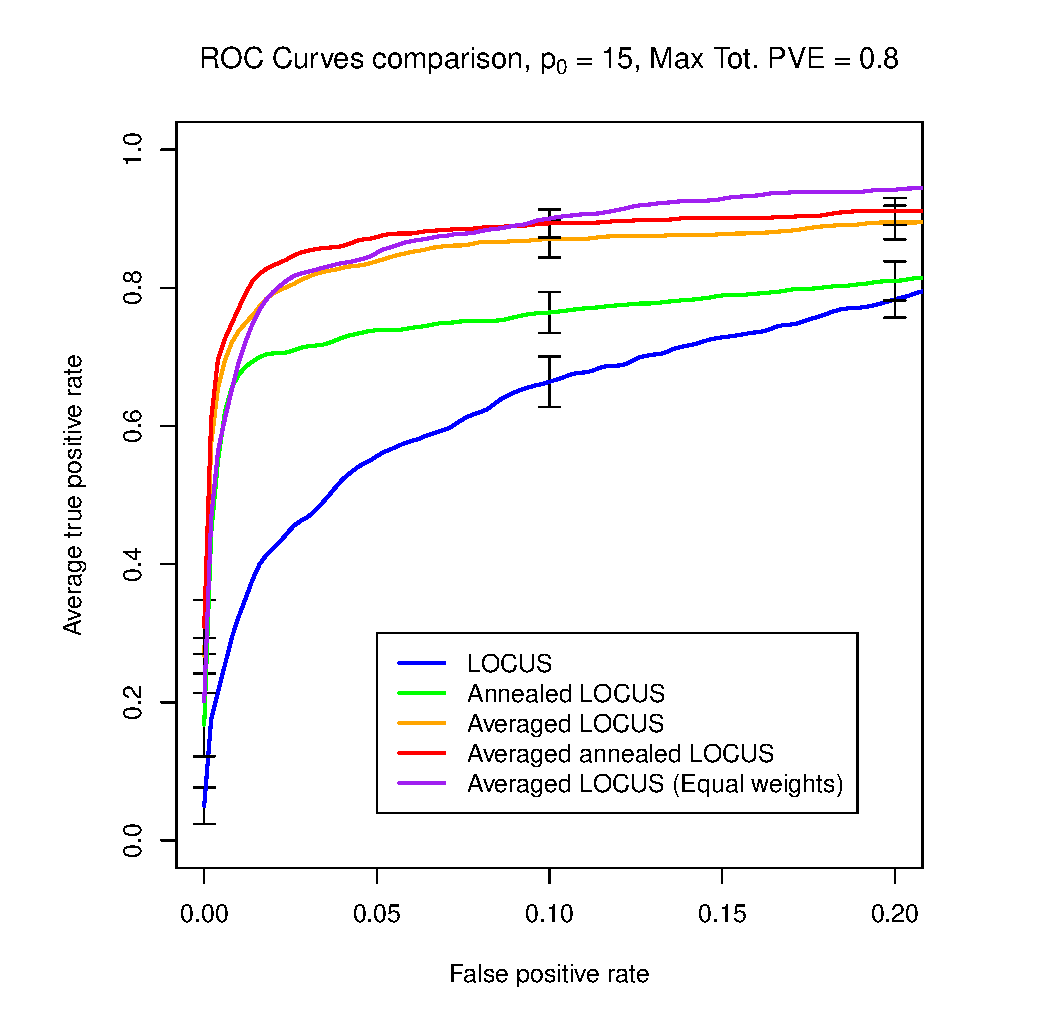
\includegraphics[width=2in]{images/ROC_curves_w_equal_weight.pdf}
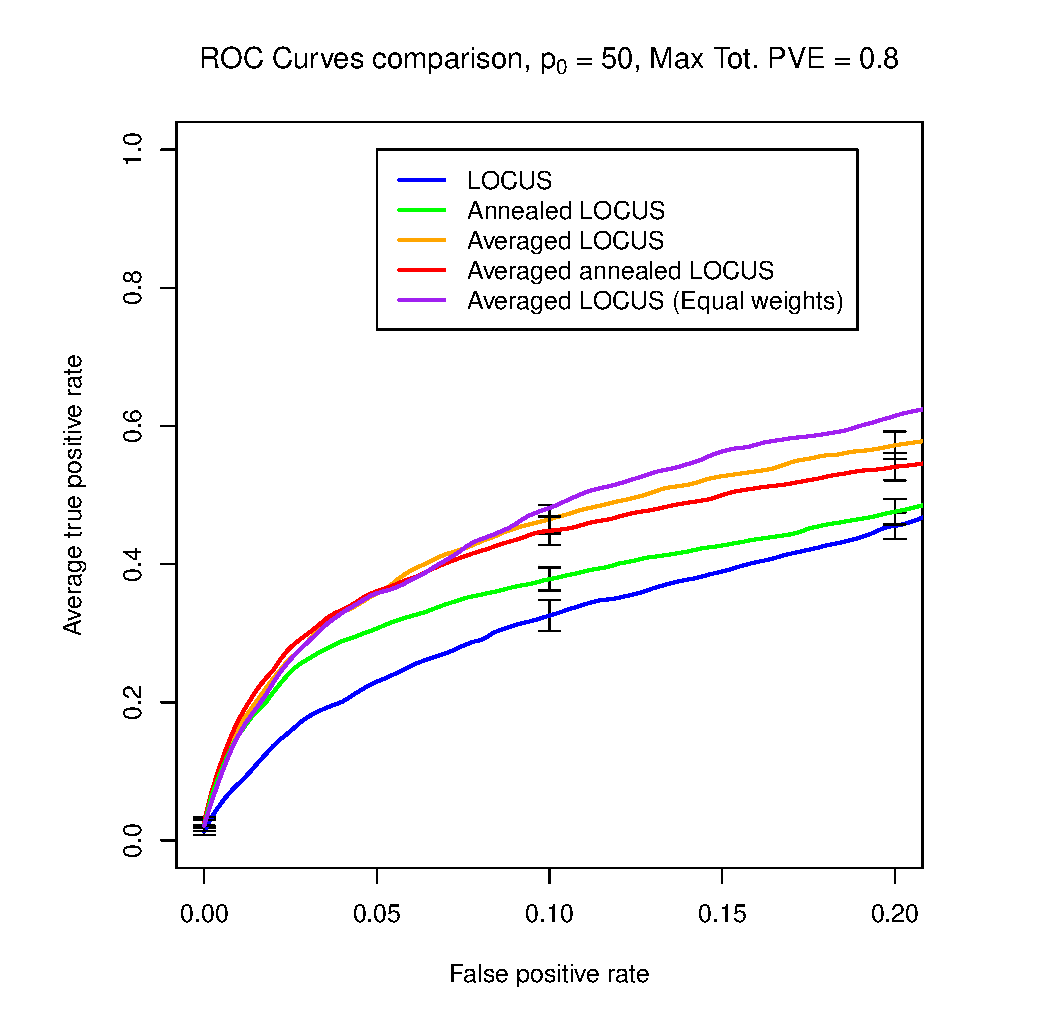
\includegraphics[width=2in]{images/ROC_curves_w_equal_weight_50.pdf}
\end{figure}
\end{frame}

\begin{frame}
\frametitle{Runtimes}
\begin{figure}
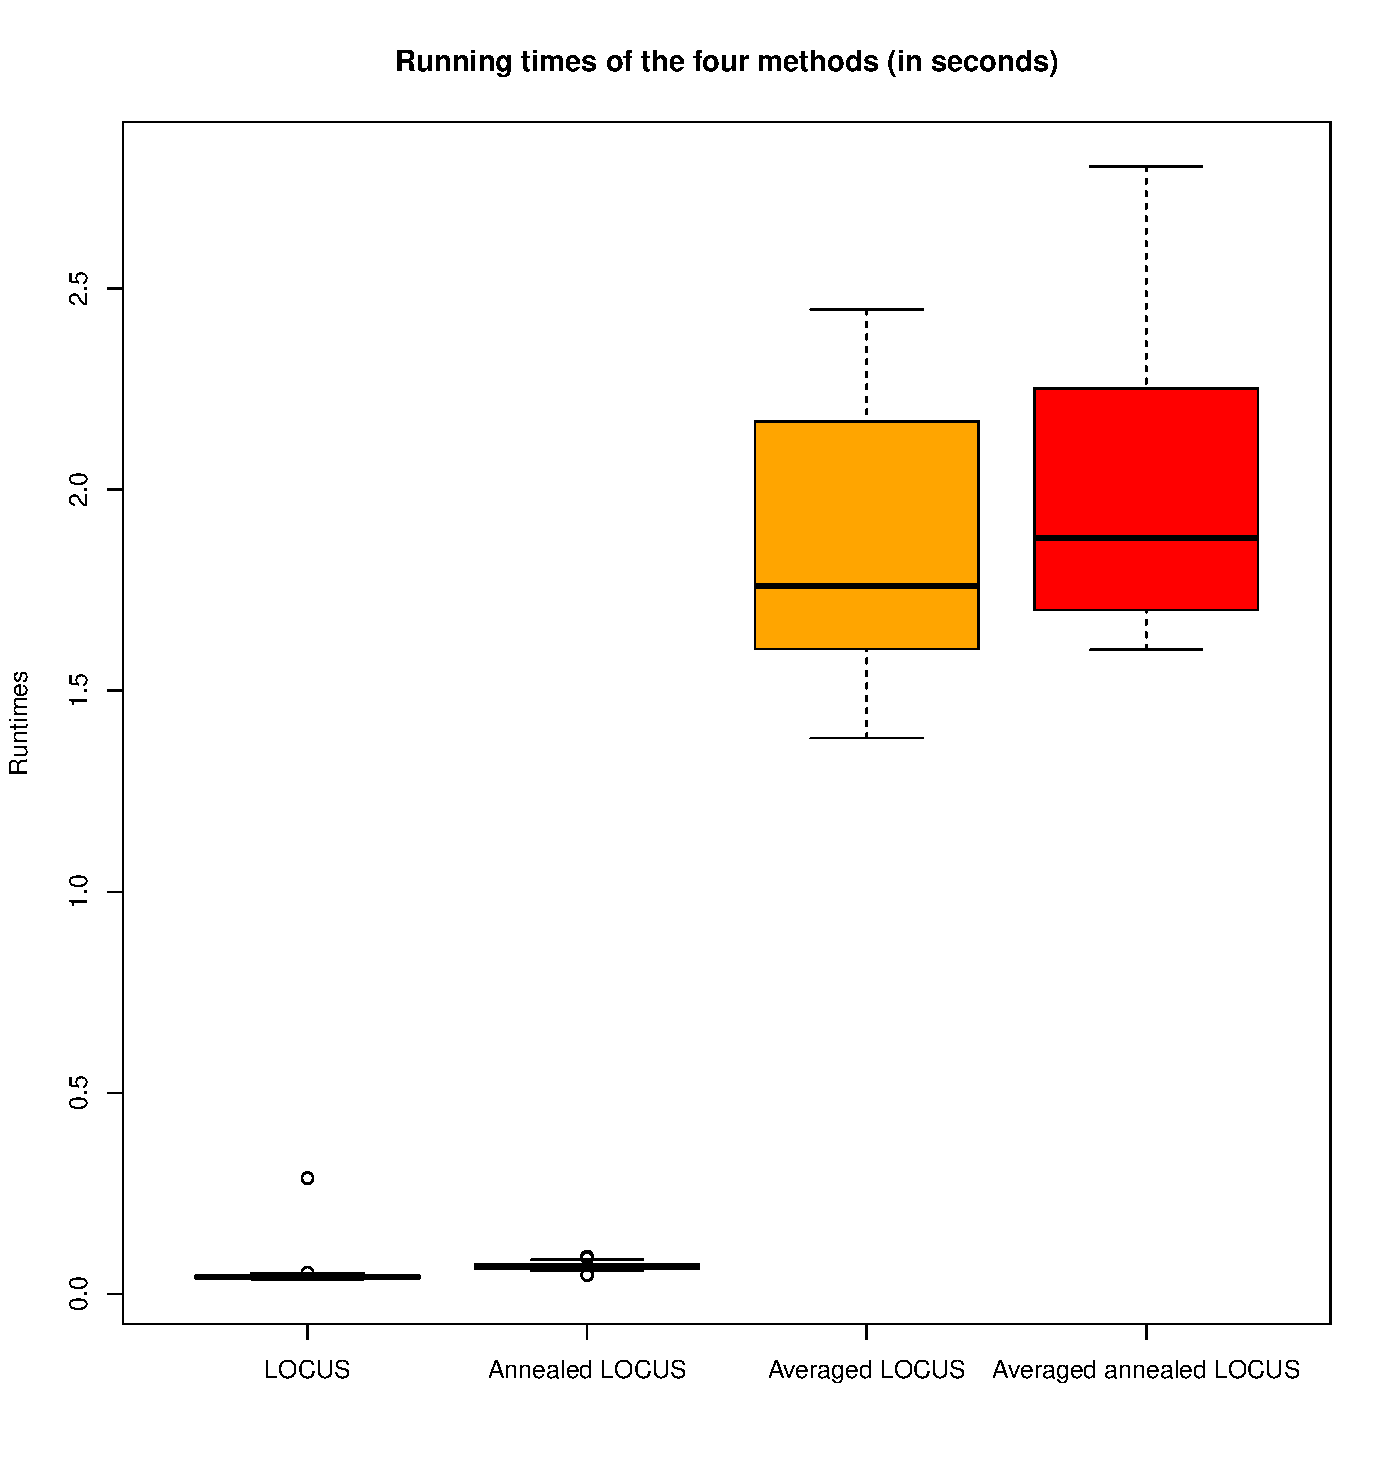
\includegraphics[width=3in]{images/runtimes.pdf}
\end{figure}
\end{frame}

%\begin{frame}
%\frametitle{Remarks}
%\begin{itemize}
%\item Paralleled computation is possible.
%\item The difference is bigger when phenotypic variance is better explained from the SNPs.
%\item The difference is bigger with fewer active SNPs.
%\end{itemize}
%\end{frame}

\begin{frame}
\frametitle{Conclusion}
\begin{itemize}
\item On strong correlated structures, Averaged LOCUS performs better than LOCUS.
\item The weights do not necessarily improve the performance.
\item Simulated annealing improves the standard LOCUS, but less the averaged LOCUS.
\end{itemize}
\end{frame}

\begin{frame}
\frametitle{Conclusion}
\begin{itemize}
\item Optimization of the code, $\rightarrow$ ev. integration to R-package,
\item Multiple traits simultaneously,
\item Application to real data.

\end{itemize}
\end{frame}

\begin{frame}
\frametitle{Thank you}
Thank you for your time.
\end{frame}
\end{document}